%Fiquemos com Deus e Nossa Senhora!
%Sao Jose de Cupertino rogai por nos!!
% ### Uses XeLaTeX ### %
% ### Needs beamer-master ### %
\documentclass[aspectratio=169]{beamer} %. Aspect Ratio 16:9

\usetheme{AI2} % beamerthemeSprace.sty
\usepackage[portuguese]{babel}
\usepackage[utf8]{inputenc}
\usepackage[T1]{fontenc}
\usepackage{ragged2e,gensymb}

\DeclareMathOperator*{\argmin}{arg\,min}
\DeclareMathOperator*{\argmax}{arg\,max}

% DATA FOR FOOTER
\date{2021}
\title{- Redes Neurais com Percepton Multicamadas}
\author{João Paulo Papa}
\institute{Advanced Institute for Artificial Intelligence (AI2)}

\begin{document}
% ####################################
% FIRST SLIDE 						:: \SliTit{This is the Title of the Talk}{A. B. Name}{Sprace}
% SUB-TITLE SLIDE 					:: \SliSubTit{<title>}{<explanation}
% SUB-SUB-TITLE SLIDE				:: \SliSubSubTit{<title>}{<explanation}
% SLIDE WITH TITLE 					:: \SliT{Title}{Content}
% SLIDE NO TITLE 						:: \Sli{Content} 
% SLIDE DOUBLE COLUMN WITH TITLE 	:: \SliDT{Title}{First Column}{Second Column}
% SLIDE DOUBLE COLUMN NO TITLE 		:: \SliD{First Column}{Second Column}
% SLIDE ADVANCED WITH TITLE 			:: \SliAdvT{Title}{Content}
% SLIDE ADVANCED NO TITLE 			:: \SliAdv{Content}
% SLIDE ADVANCED DOUBLE WITH TITLE 	:: \SliAdvDT{Title}{First Column}{Second Column}
% SLIDE ADVANCED DOUBLE NO TITLE 	:: \SliAdvD{First Column}{Second Column}
% SLIDE BLACK						:: \Black{ <Content> }
% SLIDE WHITE						:: \White{ <Content> }
% ITEMIZATION 						:: \begin{itemize}  \iOn{First} \iTw {Second} \iTh{Third} \end{itemize}
% COMMENT TEXT				 		:: \note{<comment>}
% SECTION 							:: \secx{Section} | \secxx{Sub-Section}
% BOLD SPRACE COLOR				:: \bfs{<text>}
% TABLE OF CONTENT					:: \tocitem{<title>}{<content>}
% LEFT ALIGN EQUATION				:: \begin{flalign*}  & <equation> &   \end{flalign*}
% CENTER ALIGN EQUATION	S			:: \begin{gather*} <equations>  \end{gather*}
% SLASH								:: \slashed{<>}
% BAR								:: \barr{<letter>} instead of \bar{<letter>}
% THEREFORE						:: use \portanto (larger and bold}
% 2 or 3 MATH SYMBOLS				:: \overset{<up>}{<down>} &  \underset{<below>}{\overset{<above>}{<middle>}}  
% INSERT TEXT IN FORMULA			:: \ins{<text>}
% EXERCISE							:: \exe{<exercise #>}{<exercise text>}
% SUGGESTED READING BOX			:: \sug{<references>}
% CITATION							:: \cittex{<citation>}
% CITATION DOUBLE COLUMN 			:: \cittexD{<citation>}
% TEXT POSITION						:: \texpos{<Xcm>}{<Ycm>}{<text>} origin = center of slide : x right | y down
% REFERENCE AT BOTTOM  S/D SLIDE		:: \refbotS{<reference>} \refbotD{<reference>}
% HIDDEN SLIDE						:: \hid
% COLOR BOX 						:: \blu{blue} + \red{rec} + \yel{yellow} + \gre{green} + \bege{beige}
% FRAME 							:: \fra{sprace} \frab{blue} \frar{red} + \fray{yellow} + \frag{green}		
% FIGURE 							:: \img{X}{Y}{<scale>}{Figure.png} 
% FIGURE							:: \includegraphics[scale=<scale>]{Figures/.png}
% FIGURE DOUBLE SLIDE NO TITLE		::  \img{-4}{0.5}{<scale>}{Figure.png} % Image 1st half
%									::  \img{4}{0.5}{<scale>}{Figure.png} % Image 2nd half
% FIGURE DOUBLE SLIDE WITH TITLE		::  \img{-4}{0}{<scale>}{Figure.png} % Image 1st half
%									::  \img{4}{0}{<scale>}{Figure.png} % Image 2nd half
% INCLUDING SWF (Flash)				:: \usepackage{media9} and \includemedia >> USE ACROBAT <<
%%%%%%%%%%%%%%%%%%%%%%%%%%%%%%%%%%%%%%%%%%%%%%%%%%
% ###############################################################################
% FIRST SLIDE
\SliTit{{\LARGE Redes Neurais com Percepton Multicamadas}}{Advanced Institute for Artificial Intelligence -- AI2}{https://advancedinstitute.ai}
%%%%%%%%%%%%%%%%%%%%%%%%%%%%%%%%%%%%%%%%%%%%%%%%%%
% ###############################################################################
% SLIDE SUB-TITLE
%\SliSubTit{Sub-Title}{Description}{}
%%%%%%%%%%%%%%%%%%%%%%%%%%%%%%%%%%%%%%%%%%%%%%%%%%
% ###############################################################################
%\SliSubSubTit{Sub-Sub-Title}{Description}
 %%%%%%%%%%%%%%%%%%%%%%%%%%%%%%%%%%%%%%%%%%%%%%%%%%


\SliT{Introdução}{

\justifying Redes Neurais foram amplamente utilizadas nos anos 80 e 90 e visam imitar o funcionamento do cérebro humano. Sua popularidade caiu no final dos anos 90, mas voltaram à cena com novas abordagens baseadas em aprendizado em profundidade. Mas como elas funcionam? Vamos dar uma olhada, primeiramente, na estrutura de um neurônio.

\begin{center}
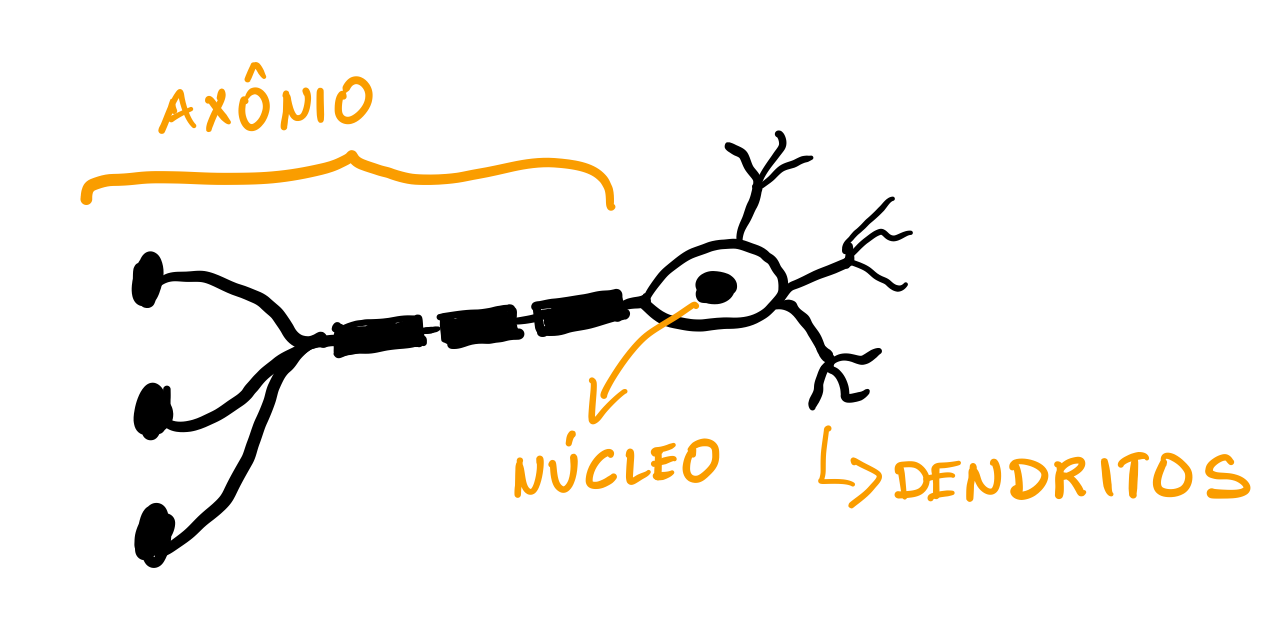
\includegraphics[scale=0.17]{./figs/Neural_Networks_Fig1.png}\hspace{1cm}
\end{center}
}

\Sli{
Matematicamente falando, podemos representar um neurônio da seguinte forma (Modelo de McCulloch-Pitts):

\begin{center}
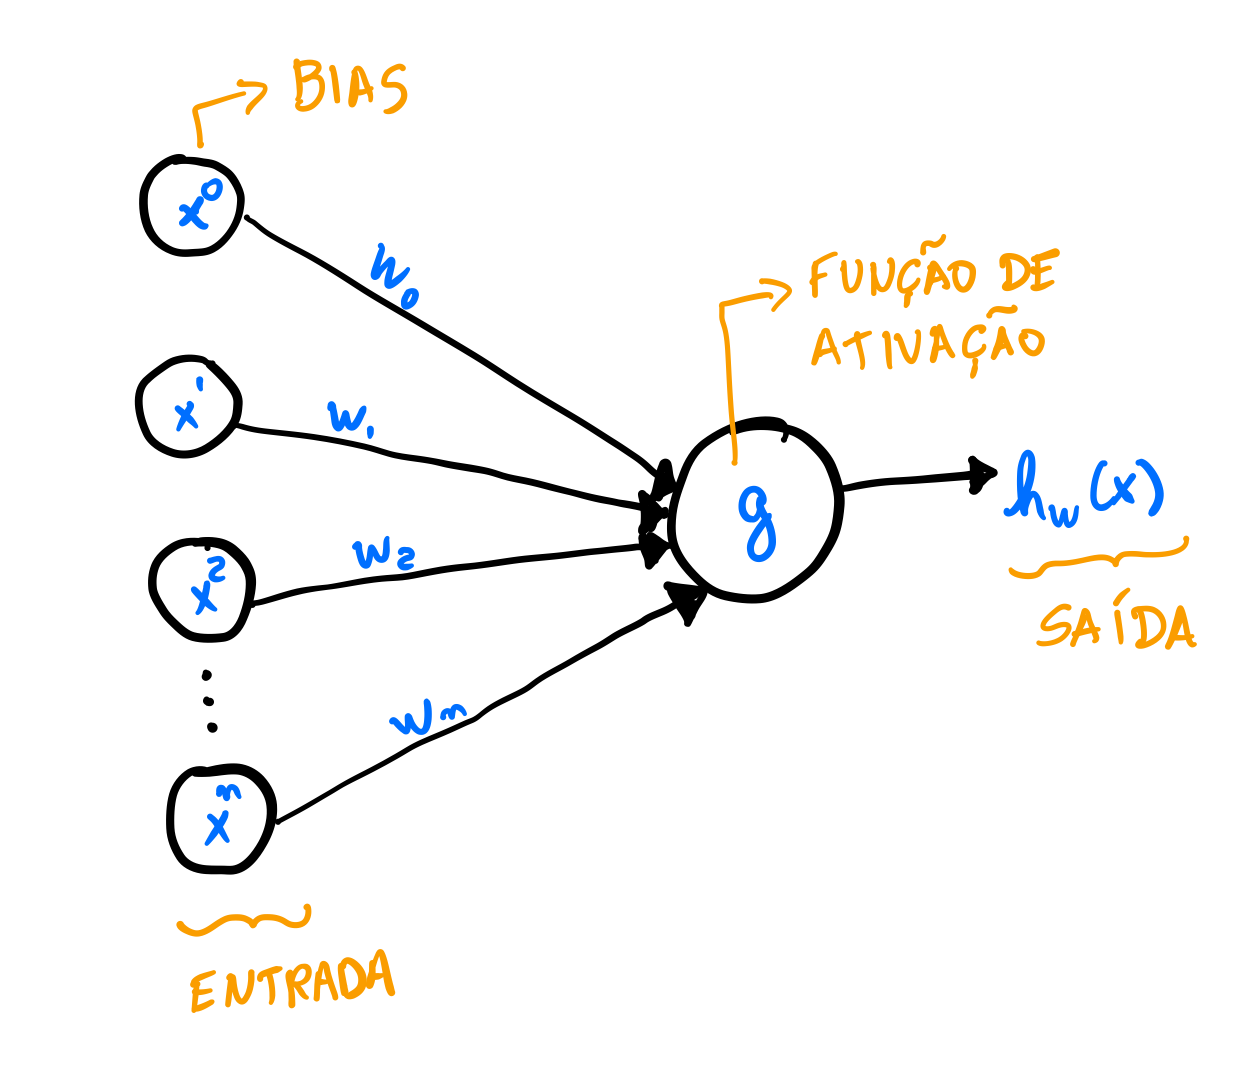
\includegraphics[scale=0.15]{./figs/Neural_Networks_Fig2.png}\hspace{1cm}
\end{center}
}

\Sli{
Alguns exemplos de funções de ativação:

\begin{itemize}
	\item Função logística (sigmoide): $g(a) = \frac{1}{1+e^{-a}}$, tal que $g(a)\in[0,1]$.
	\item Função limiar (degrau): 
	\begin{equation}\nonumber
		g_{\theta}(a) = 
		\begin{cases}
		1\text{ caso } \boldsymbol{w}^T\boldsymbol{x} \geq \theta\\
		0\text{ caso contrário}.
		\end{cases}
	\end{equation}
	tal que $g(a)\in\{0,1\}$.
	\item Função tangente hiperbólica: $g(a) = 2\sigma(2a)-1$, tal que $g(a)\in[-1,1]$ e $\sigma(x)$ corresponde à função logística.
\end{itemize}
}

\Sli{
É desejável que uma função de ativação seja \textbf{derivável}. Como escolhê-la? Depende de sua aplicação.

\begin{minipage}{0.49\textwidth}
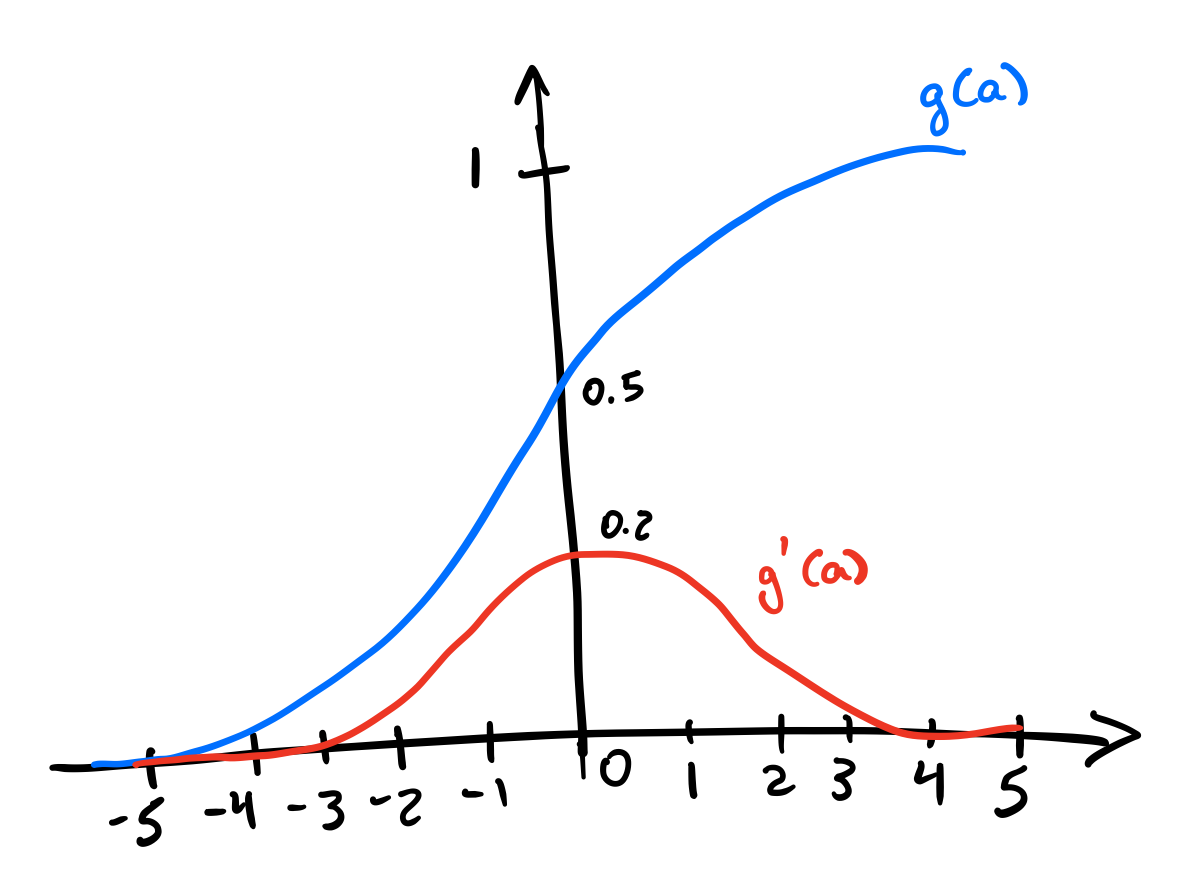
\includegraphics[scale=0.17]{./figs/Neural_Networks_Fig3.png}
\end{minipage}%%% to prevent a space
\begin{minipage}{0.37\textwidth}
Suponha $g(a) = \frac{1}{1+e^{-a}}$. Temos que $g^\prime(a) = g(a)(1-g(a))$. Note que $g^\prime(a)$ satura quando $a>5$ ou $a<-5$. Ademais, $g^\prime(a) <1$, $\forall a$. Isso significa que, para redes com muitas camadas, o gradiente tende a \textbf{desaparecer} durante o treinamento. 
\null
\par\xdef\tpd{\the\prevdepth}
\end{minipage}
}

\Sli{
\begin{minipage}{0.49\textwidth}
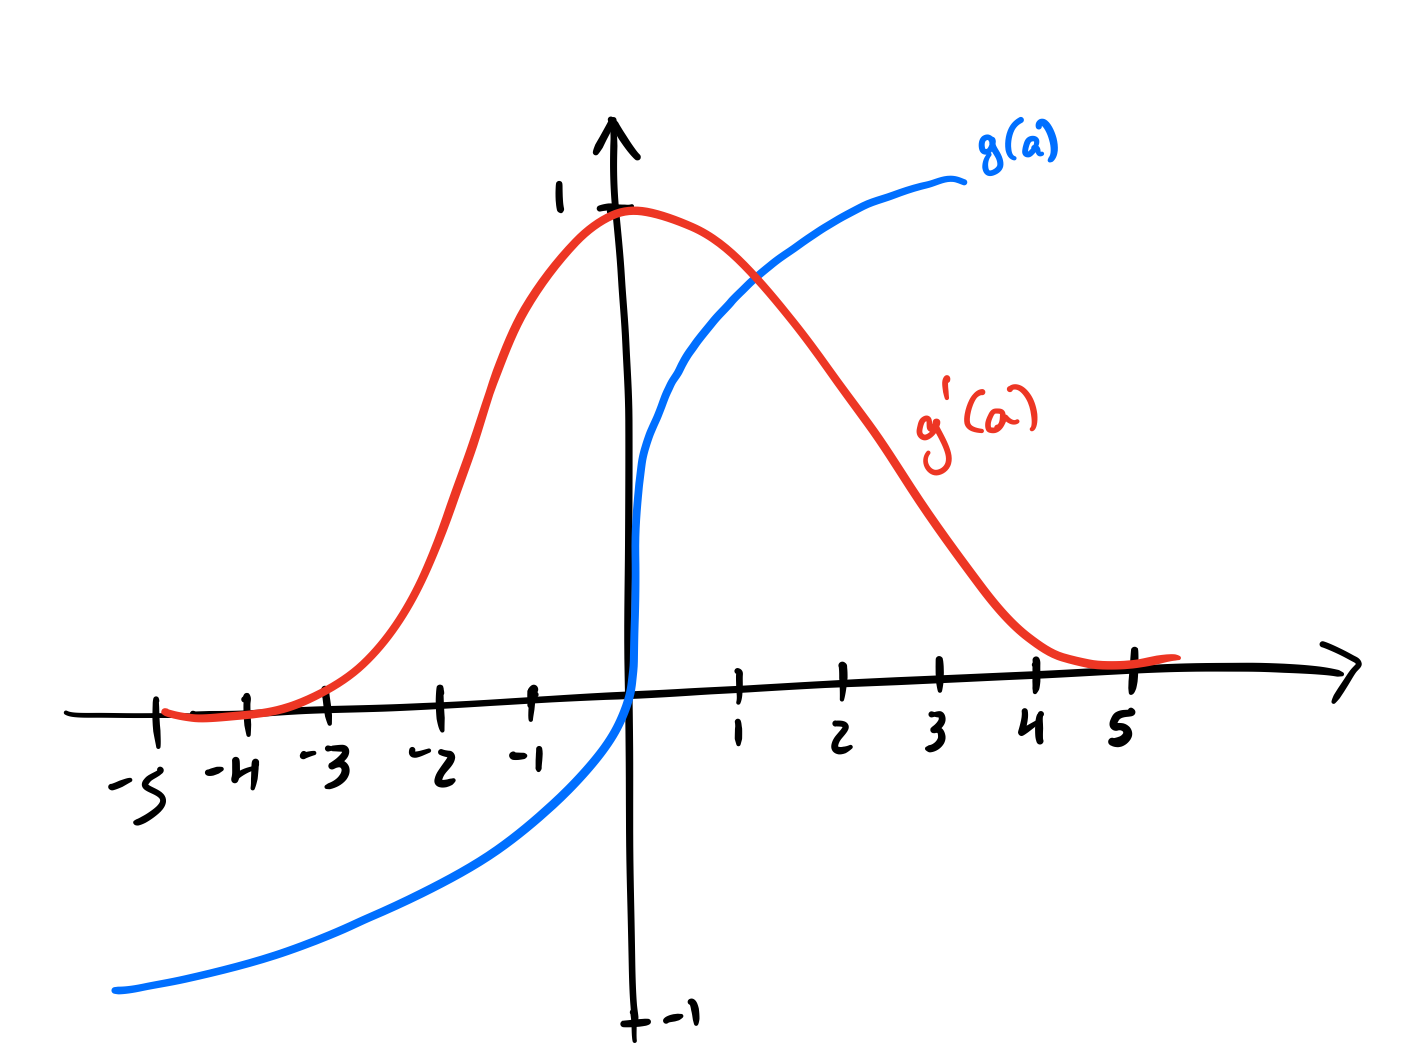
\includegraphics[scale=0.15]{./figs/Neural_Networks_Fig4.png}
\end{minipage}%%% to prevent a space
\begin{minipage}{0.37\textwidth}
Suponha $g(a) = 2\sigma(2a)-1$. Temos que $g^\prime(a) = 1-g^2(a)$. Muito embora saturações aconteçam, $g^\prime(a)$ atinge valores maiores, chegando, inclusive, ao máximo de $1$ quando $a=0$.
\null
\par\xdef\tpd{\the\prevdepth}
\end{minipage}
}

\Sli{
\secx{Perceptron}

\justify O Perceptron foi formalmente proposto por McCulloch e Pitts na década de 40 com o intuito de modelar matematicamente o neurônio humano. Muito embora ele tenha sido a base para muitos algoritmos, seu poder discriminativo é limitado, pois consegue aprender apenas hiperplanos como função de decisão.

\justify \underline{Definição do problema:} seja um conjunto de dados ${\cal X}= \{(\boldsymbol{x}_1,y_1),(\boldsymbol{x}_2,y_2),\ldots,(\boldsymbol{x}_z,y_z)\}$ tal que $\boldsymbol{x}_i\in\mathbb{R}^{n+1}$ corresponde ao dado de entrada e $y_i\in[0,1]$ denota o seu respectivo valor de saída. Temos, ainda, que ${\cal X}$ pode ser \textbf{particionado} da seguinte forma: ${\cal X} = {\cal X}^1\cup {\cal X}^2$, em que ${\cal X}^1$ e ${\cal X}^2$ denotam os conjuntos de dados de \textbf{treinamento} e \textbf{teste}, respectivamente. Nosso objetivo é, dado o conjunto de treinamento, aprender uma função $h:\mathbb{R}^{n+1}\rightarrow\{0,1\}$ que consiga atribuir a classe correta à uma determinada amostra.
}

\Sli{
Vamos, agora, adaptar a função de ativação limiar para que possamos criar a nossa função hipótese:

\begin{equation}
	h_{\boldsymbol{w}}(\boldsymbol{x}) = 
	\begin{cases}
		1\text{ caso }\boldsymbol{w}^T\boldsymbol{x}\geq \theta\\
		0\text{ caso contrário.}
	\end{cases}
\end{equation}

Para simplificar a notação, é usual trazermos $\theta$ para o lado esquerdo da equação e atribuirmos $w_0=\theta$. Novamente, consideraremos $x^0=1$. Assim, temos a função hipótese atualizada como segue:

\begin{equation}
	h_{\boldsymbol{w}}(\boldsymbol{x}) = 
	\begin{cases}
		1\text{ caso }\boldsymbol{w}^T\boldsymbol{x}\geq 0\\
		0\text{ caso contrário.}
	\end{cases}
\end{equation}
}

\Sli{
Vamos, agora, revisitar alguns conceitos de Geometria Analítica. Suponha que tenhamos dois vetores $\boldsymbol{u} = [u_1\ u_2]$ e $\boldsymbol{v} = [v_1\ v_2]$. Geometricamente, podemos representá-los como segue:

\begin{minipage}{0.49\textwidth}
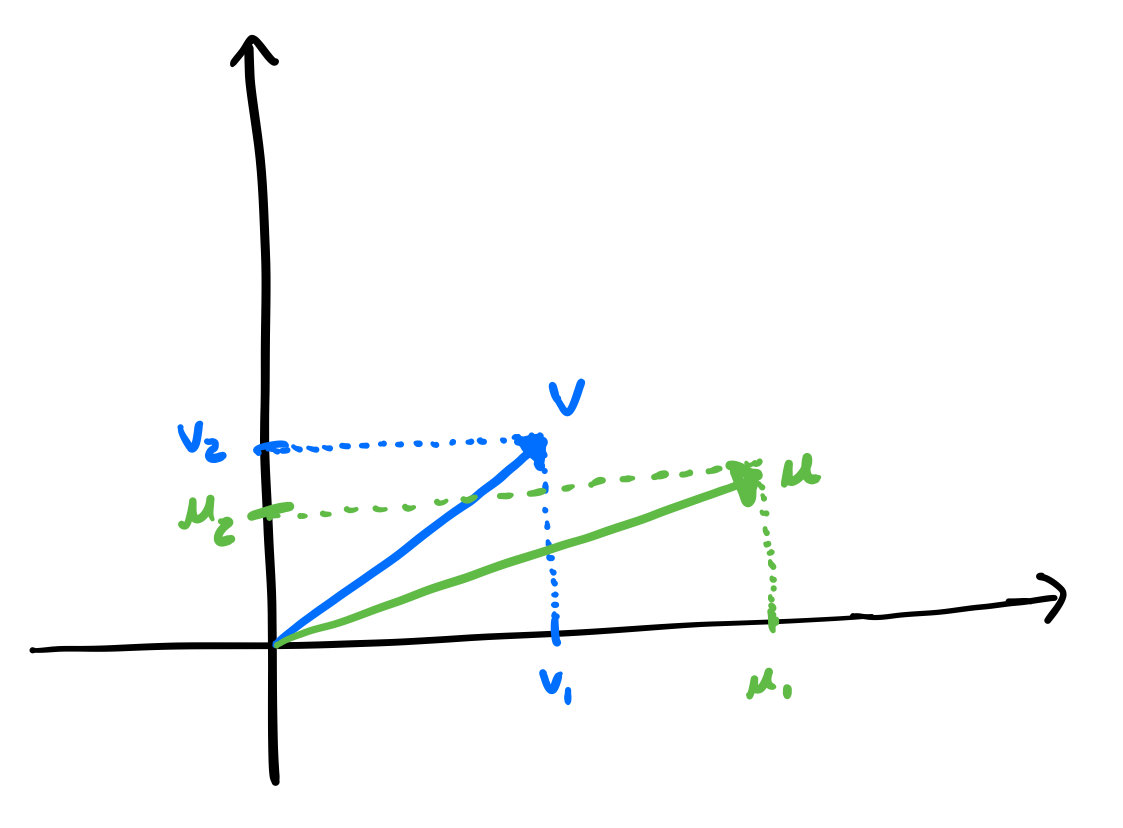
\includegraphics[scale=0.17]{./figs/Neural_Networks_Fig5.png}
\end{minipage}%%% to prevent a space
\begin{minipage}{0.37\textwidth}
Lembrando que $\norm{u} = \sqrt{u_1^2+u_2^2}$ denota o comprimento (magnitude) de $u$.
\null
\par\xdef\tpd{\the\prevdepth}
\end{minipage}
}

\Sli{
Temos, também, a definição de \textbf{projeção escalar} entre dois vetores, dada como segue:

\begin{minipage}{0.49\textwidth}
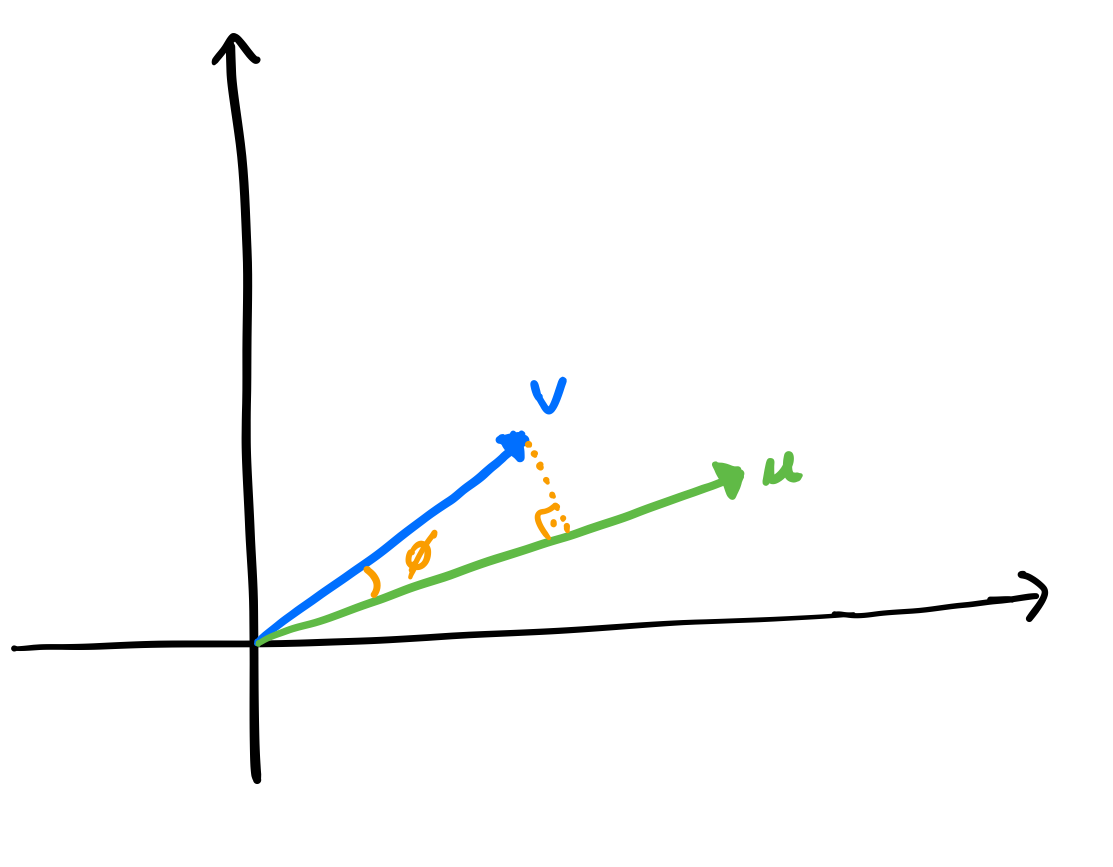
\includegraphics[scale=0.17]{./figs/Neural_Networks_Fig6.png}
\end{minipage}%%% to prevent a space
\begin{minipage}{0.37\textwidth}
Podemos, então, representar o produto escalar entre dois vetores da seguinte forma: $\boldsymbol{w}^T\boldsymbol{x} = \norm{\boldsymbol{w}}.\cos\phi$. Lembrando que temos as seguintes situações:

	\begin{itemize}
		\item $\cos\phi > 0$ quando $\phi < 90\degree$.
		\item $\cos\phi < 0$ quando $\phi > 90\degree$.
		\item $\cos\phi = 0$ quando $\phi = 90\degree$ 
	\end{itemize}
	
\null
\par\xdef\tpd{\the\prevdepth}
\end{minipage}
}

\Sli{
Voltando ao nosso problema inicial, temos que a equação $\boldsymbol{w}^T\boldsymbol{x}=0$ define um hiperplano normal ao vetor de pesos $\boldsymbol{w}$ deslocado de $-\theta$ (assumindo que $w_0=-\theta$ e $x_0 = 1$). Vamos supor 	que $\theta = 0$, ou seja, o hiperplano passa pela origem.
}

\begin{center}
	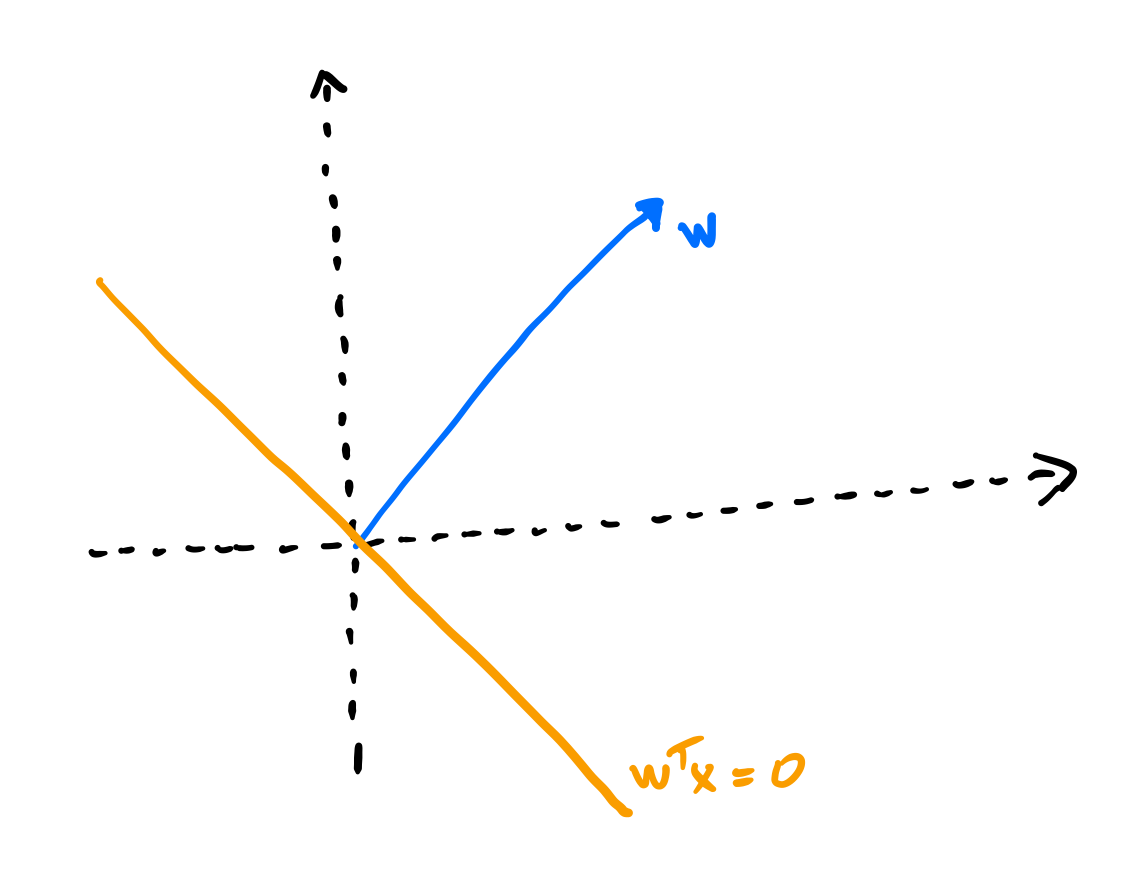
\includegraphics[scale=0.17]{./figs/Neural_Networks_Fig7.png}
\end{center}

\end{document}